\documentclass[xcolor=table]{beamer}

\usepackage[french]{babel}
\usepackage[latin1]{inputenc}
\usepackage[normalem]{ulem}
\usepackage[T1]{fontenc}
\usepackage{fancyhdr}   %% Pour la gestion des num�ros de page
\usepackage{graphicx}
\usepackage{amsmath}
\usepackage{mathrsfs}
\usepackage{amsfonts}
\usepackage{palatino}        %% Palatino fonts
\usepackage{mathptm}        %% PostScript Type 1 math fonts
\usepackage{dsfont} %% Pour mathds
\usepackage{color}
%%\usepackage{pstricks}
\usepackage{xmpmulti}
\usepackage{hyperref}
\usepackage{multimedia}
\usepackage{multirow}
%\usepackage[table]{xcolor}
\usepackage{fourier-orns}
\usepackage{subfigure}
\usepackage{tikz}

\DeclareMathAlphabet{\mathpzc}{OT1}{pzc}{m}{it}

\definecolor{vert}{rgb}{0.07,0.7,0.00}
\definecolor{gris}{gray}{0.70}
\definecolor{gris2}{gray}{0.95}
\definecolor{bleu}{rgb}{0.19,0.19,0.68}

%table setting
\newcommand\T{\rule{0pt}{2.6ex}}
\newcommand\B{\rule[-1.2ex]{0pt}{0pt}}
\renewcommand{\thesubfigure}{\thefigure.\arabic{subfigure}}

\usetheme{allee_marine} %voir fichier beaerthemeallee_marine.sty   ==> \usetheme{allee_marine}


%%%%%%%%%%%%%%%%%%%%%%%%%% Pr�sentation du document %%%%%%%%%%%%%%%%%%%%%%%%%%
\title[Master 1 Project]{Indexing big colored image bank : Texture 3.0}
\author[Etienne CAILLAUD, Thomas LE BRIS, Ibrahima GUEYE, Gaetan ADIER]{\textbf{Etienne CAILLAUD, Thomas LE BRIS, Ibrahima GUEYE, Gaetan ADIER}}
\institute [XLIM-SIC UMR CNRS 7252]{\textbf{XLIM-SIC Laboratory UMR CNRS 7252, Poitiers, France}}
\date{}

%%%%%%%%%%%%%%%%%%%%%%% Num�ro de pages en bas � gauche %%%%%%%%%%%%%%%%%%%%%%
\addtobeamertemplate{footline}{\color{blue}\hfill\insertframenumber/\inserttotalframenumber}

\pgfdeclareimage[height=96mm,width=128mm]{nombidon}{Fond}
\setbeamertemplate{background}{\pgfuseimage{nombidon}}

\pgfdeclareimage[height=96mm,width=128mm]{nombidon2}{Fond}
\setbeamertemplate{background}{\pgfuseimage{nombidon2}}

%%----------------------------------------------------------------------------
%% A chaque d�but de sous-section : g�n�re une table des mati�res
%%----------------------------------------------------------------------------
\AtBeginSection[]
{
   \setbeamertemplate{background}{\pgfuseimage{nombidon}}
   \begin{frame}<beamer>
    \frametitle{Outline}
    \tableofcontents[currentsection, hideallsubsections] %% affiche la section courante et les autres en gris�, masque les sous-sections
   \end{frame}
  \setbeamertemplate{background}{\pgfuseimage{nombidon2}}
}

\AtBeginSubsection[]
{
  \setbeamertemplate{background}{\pgfuseimage{nombidon}}
  \begin{frame}<beamer>
    \tableofcontents[sectionstyle=show/shaded,subsectionstyle=show/shaded/hide, subsubsectionstyle =hide]
  \end{frame}
   \setbeamertemplate{background}{\pgfuseimage{nombidon2}}
}

\AtBeginSubsubsection[]
{
  \setbeamertemplate{background}{\pgfuseimage{nombidon}}
  \begin{frame}<beamer>
    \tableofcontents[sectionstyle=show/shaded,subsectionstyle=show/shaded/hide,subsubsectionstyle =show/shaded/hide]
  \end{frame}
   \setbeamertemplate{background}{\pgfuseimage{nombidon2}}
}


%%%%%%%%%%%%%%%%%%%%%%%%%%%%%%%%%%%%%%%%%%%%%%%%%%%%%%%%%%%%%%%%%%%%%%%%%%%%%%
%%%%%%%%%%%%%%%%%%%%%%%%%%%%                       %%%%%%%%%%%%%%%%%%%%%%%%%%%
%%%%%%%%%%%%%%%%%%%%%%%%%%     DEBUT DU DOCUMENT     %%%%%%%%%%%%%%%%%%%%%%%%%
%%%%%%%%%%%%%%%%%%%%%%%%%%%%                       %%%%%%%%%%%%%%%%%%%%%%%%%%%
%%%%%%%%%%%%%%%%%%%%%%%%%%%%%%%%%%%%%%%%%%%%%%%%%%%%%%%%%%%%%%%%%%%%%%%%%%%%%%
\begin{document}
\graphicspath{{images/}}
\setbeamercolor{block title example}{bg = gray}

\begin{frame}
    \vspace{-1.5cm}
    \begin{tikzpicture}[remember picture,overlay]
        \node[xshift=0cm, above=8.6cm] at (current page.south west)
        {
\includegraphics[width=40cm,height=0.9cm]{cache_titre.png}};
        \node[xshift=2cm, above=2.8cm] at (current page.south west)
        {
\includegraphics[height=1.5cm]{Xlim.png}};
        \node[xshift=11cm, above=3cm] at (current page.south west)
        {
\includegraphics[height=1cm]{logo_une.jpg}};
        \node[xshift=6.5cm, above=0.7cm] at (current page.south west)
        {
\includegraphics[height=1.6cm]{Lifeclef.png}};
    \end{tikzpicture}
    \titlepage
\end{frame}

%%%%%%%%%%%%%%%%%%%%%%%%%%%%%%%%%%%%%%%%%%%%%%%%%%%%%%%%%%%%%%%%%%%%%%%%%%%%%%%%%%%%%%%%%%%%%%%%%%%%%
%%%%%%%%%%%                     D�but de la pr�sentation                       	     		 %%%%%%%%
%%%%%%%%%%%%%%%%%%%%%%%%%%%%%%%%%%%%%%%%%%%%%%%%%%%%%%%%%%%%%%%%%%%%%%%%%%%%%%%%%%%%%%%%%%%%%%%%%%%%%
\section{Introduction to the project context}
%%-----------------------------------------------------------------------------------------
%%-----------------------------------------------------------------------------------------
\begin{frame} \frametitle{Project context (1/3)}
%%-----------------------------------------------------------------------------------------
%% objective + image index
%%-----------------------------------------------------------------------------------------
\begin{block}{Objective}
  Test a solution for content based image indexing flaw : standard descriptors (SIFT, SURF, etc) lacking real color and texture information.
\end{block} :
	
\begin{figure}
	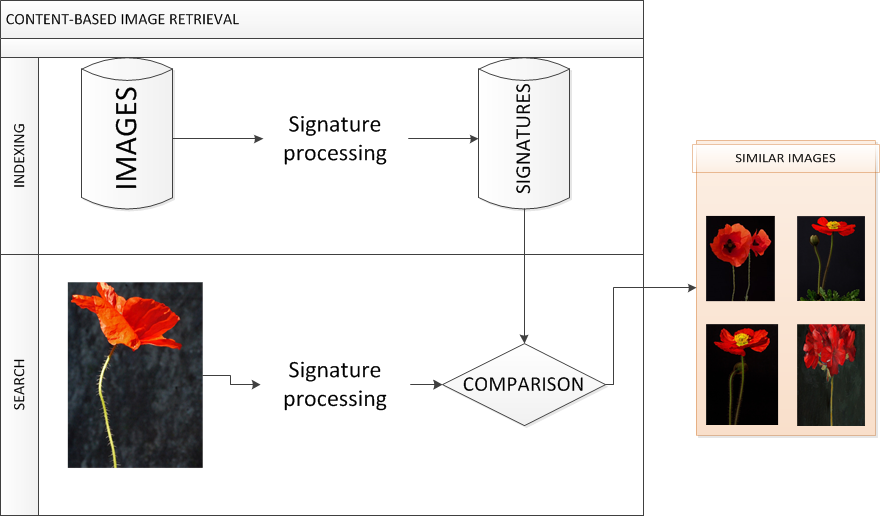
\includegraphics{CBIR.png}
\end{figure}



\end{frame}
%%-----------------------------------------------------------------------------------------

\begin{frame} \frametitle{Project context 2/3}
%%-----------------------------------------------------------------------------------------
%% Image Indexing
%%-----------------------------------------------------------------------------------------
\begin{block}{What is a descriptor ?}
	Algorithm applied to an image which output is a short vector
	of numbers which is invariant to common image transformations
	and can be compared with other descriptors in a	database.
\end{block} :


\begin{figure}
   \begin{minipage}[c]{.46\linewidth}
      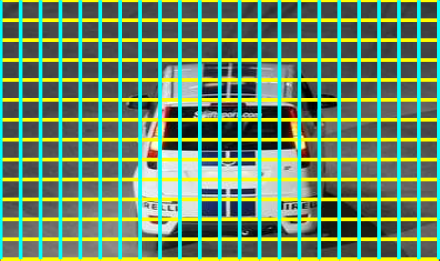
\includegraphics{dense_grid.png}
	  \caption Densegrid
   \end{minipage} \hfill
   \begin{minipage}[c]{.46\linewidth}
      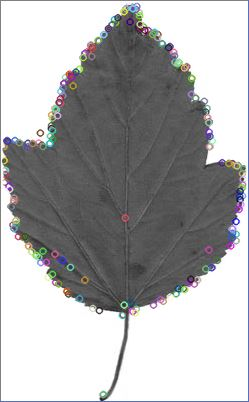
\includegraphics{siftKP.jpg}
	  \caption Interest points
   \end{minipage}
\end{figure}





\end{frame}
%%-----------------------------------------------------------------------------------------

\begin{frame} \frametitle{Project context 3/3}
%%-----------------------------------------------------------------------------------------
%% Parler de clef, des traitements couleurs marginaux ??}
%%-----------------------------------------------------------------------------------------
\begin{block}{What is a CLEF ?}
	International contest which purpose is to provide a place where labs and companies solution for multimedia analysis of life can compete against each other.
\end{block} :

\begin{figure}

\end{figure}
	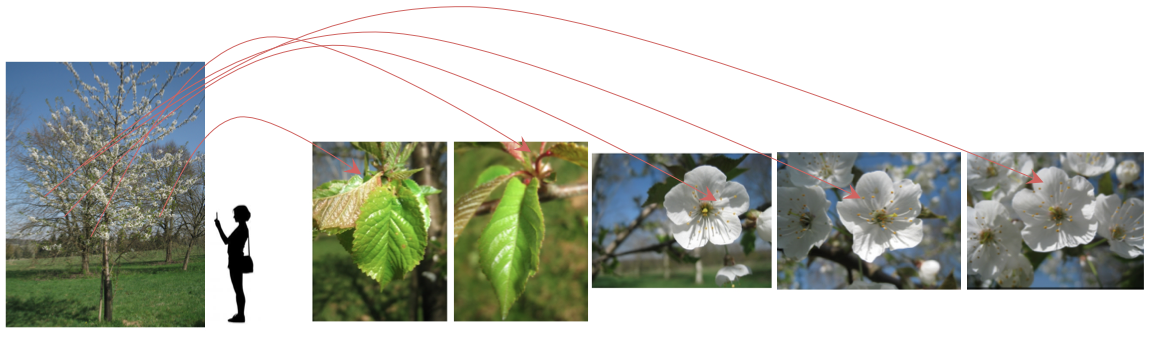
\includegraphics{OnePrunus.png}
\end{frame}
%%-----------------------------------------------------------------------------------------


\begin{frame} \frametitle{Team presentation}
%%-----------------------------------------------------------------------------------------

% Schema demande par mr Richard
\end{frame}
%%-----------------------------------------------------------------------------------------


\begin{frame} \frametitle{User requirement}
%%-----------------------------------------------------------------------------------------

% Parler de la demande de base, ce qui etait convenu avec le client ...
\end{frame}
%%-----------------------------------------------------------------------------------------


\section{Work and results}

\begin{frame} \frametitle{SIFT (1/2)}
%%-----------------------------------------------------------------------------------------

\end{frame}
%%-----------------------------------------------------------------------------------------

\begin{frame} \frametitle{SIFT (2/2)}
%%-----------------------------------------------------------------------------------------

\end{frame}
%%-----------------------------------------------------------------------------------------



\begin{frame} \frametitle{C$_2$O (1/4)}
%%-----------------------------------------------------------------------------------------

% Commencer par l'interet des C2O par rapport aux autres descripteurs, (difference entre traitement vectoriel et marginal)

\end{frame}
%%-----------------------------------------------------------------------------------------


\begin{frame} \frametitle{C$_2$O (2/4)}
%%-----------------------------------------------------------------------------------------

% Repprendre la premiere diapo en remplacant Lab par "perceptual space" et mettre les refs d'articles sur le lab en footnotes

\end{frame}
%%-----------------------------------------------------------------------------------------



\begin{frame} \frametitle{C$_2$O (3/4)}
%%-----------------------------------------------------------------------------------------

% Mettre des exemples de matrice C2O sur des images de la base qui seront parlant !!

\end{frame}
%%-----------------------------------------------------------------------------------------


\begin{frame} \frametitle{C$_2$O (4/4)}
%%-----------------------------------------------------------------------------------------

% Mettre en petit en haut l'illustration coords spheriques et montrer les signatures correspondant aux matrices

\end{frame}
%%-----------------------------------------------------------------------------------------




\begin{frame} \frametitle{Bag of word}
%%-----------------------------------------------------------------------------------------

% Mettre un exemple equivalent avec 4 classes : puis faire apparaitres clairement les points a ressortir
% Expliquer le principe des k-means
% Montrer et expliquer les histogrammes de mots

\end{frame}
%%-----------------------------------------------------------------------------------------


\begin{frame} \frametitle{k-nn}
%%-----------------------------------------------------------------------------------------

% Garder ce qui a �t� fait, notifier le fait que le point noir soit la donnee a classifier

\end{frame}
%%-----------------------------------------------------------------------------------------




\begin{frame} \frametitle{Result and discussion (1/2)}
%%-----------------------------------------------------------------------------------------

% Mettre un fond color� pour les case ou le resultat est le m�me que pour le sift

\end{frame}
%%-----------------------------------------------------------------------------------------

\begin{frame} \frametitle{Result and discussion (2/2)}
%%-----------------------------------------------------------------------------------------

% Discussion : parler de l'impact des parametres (Norme de delta en fct de l'image, distance pas forcement bonne, ordre de concatenation pas bon,...)

\end{frame}
%%-----------------------------------------------------------------------------------------


%%-----------------------------------------------------------------------------------------
\section{Project management}
%%-----------------------------------------------------------------------------------------



\begin{frame} \frametitle{Scheduling}
%%-----------------------------------------------------------------------------------------

% Montrer le passage d'un gantt a un backlog produit, => mettre l'accent sur la modification du gantt sans modification du backlog notable
\end{frame}
%%-----------------------------------------------------------------------------------------

\begin{frame} \frametitle{Project gestion}
%%-----------------------------------------------------------------------------------------

% Gestion par sprint : ????
\end{frame}
%%-----------------------------------------------------------------------------------------

\begin{frame} \frametitle{Our experience}
%%-----------------------------------------------------------------------------------------

% Complique? Utile ?
\end{frame}
%%-----------------------------------------------------------------------------------------



%%-----------------------------------------------------------------------------------------
\section{Conclusion}
%%-----------------------------------------------------------------------------------------


\begin{frame} \frametitle{Objectives}
%%-----------------------------------------------------------------------------------------

% Rappel des objectifs de base
\end{frame}
%%-----------------------------------------------------------------------------------------


\begin{frame} \frametitle{Achieved work}
%%-----------------------------------------------------------------------------------------

% Rappel des objectifs de base
\end{frame}
%%-----------------------------------------------------------------------------------------


\begin{frame} \frametitle{Problem encountered}
%%-----------------------------------------------------------------------------------------
%
\end{frame}
%%-----------------------------------------------------------------------------------------


\begin{frame} \frametitle{Personal point of view}
%%-----------------------------------------------------------------------------------------

% Rappel des objectifs de base
\end{frame}
%%-----------------------------------------------------------------------------------------






\section{}
\begin{frame}\frametitle{}
%%-----------------------------------------------------------------------------------------
    \begin{center}
        Thanks for attention
    \end{center}
\end{frame}
%%-----------------------------------------------------------------------------------------


\end{document}

